
\mychapter{Introduction}

\thispagestyle{empty}
\frenchspacing

\section{The Śivadharma corpus}
\fancyhead[CE]{{\footnotesize \textit{Vṛṣasārasaṃgraha}}}
\fancyhead[CO]{{\footnotesize \textit{Introduction}}}
\fancyhead[LE]{}
\fancyhead[RE]{}
\fancyhead[LO]{}
\fancyhead[RO]{}

In general...

\section{Reading the \Vsssc}

\subsection{The title}
The title \Vss\ can be translated as:
`A Compendium on the Essence of the Bull [of Dharma].'
The last two elements (\skt{sāra-saṃgraha}) need
little explanation: this work is a 
`compendium' on, a `collection' or `summary' of (\skt{saṃgraha})
the `essence' (\skt{sāra}) of its topic. The words 
`compendium' and `collection' reflect the composite nature of
the \Vss\ well; see sections on the structure of the text and
on the its possible sources on pp. ??ff and pp. ??ff.
The remaining question is weather the bull in the title 
is only a reference to a representation of Dharma 
or also a hint at Śiva's bull, his vehicle or mount, 
sometimes called Nandi or Nandin in other works.%
		\footnote{There is no trace of Nandi/Nandin
		as identified with the bull in the \Vss.
		On the possible time after which 
		Nandi or Nandin, originally a \cskt{gaṇa}{gana} 
		was considered a \csindex{bull}, see 
		\mycite{bhattacharya_nandin_1977} and 
		\mycitep{Pancavaranastava}{100--108 and 171--172}.}

Dharma is frequently referred to as a (four-legged) 
bull in Sanskrit literature from at least the time of the \MBh. 
See, e.g., this passage (\MBH\ 3.188.10--13):

\begin{quote}
{\small
  \skt{kṛte \textbf{catuṣpāt} sakalo nirvyājopādhivarjitaḥ} |\\
  \skt{vṛṣaḥ pratiṣṭhito dharmo manuṣyeṣv abhavat purā} || 10 ||\\
  \skt{adharmapādaviddhas tu tribhir aṃśaiḥ pratiṣṭhitaḥ} |\\
  \skt{tretāyāṃ dvāpare 'rdhena vyāmiśro dharma ucyate} || 11 ||\\
  \skt{tribhir aṃśair adharmas tu lokān ākramya tiṣṭhati} |\\
  \skt{caturthāṃśena dharmas tu manuṣyān upatiṣṭhati} || 12 ||\\
  \skt{āyur vīryam atho buddhir balaṃ tejaś ca pāṇḍava} |\\
  \skt{manuṣyāṇām anuyugaṃ hrasatīti nibodha me} || 13 ||\\
  }
\end{quote}

Śiva got his bull, MBh:
13076027a vṛṣabhaṃ ca dadau tasmai saha tābhiḥ prajāpatiḥ
13076027c prasādayām āsa manas tena rudrasya bhārata
13076028a prītaś cāpi mahādevaś cakāra vṛṣabhaṃ tadā
13076028c dhvajaṃ ca vāhanaṃ caiva tasmāt sa vṛṣabhadhvajaḥ
13076029a tato devair mahādevas tadā paśupatiḥ kṛtaḥ
13076029c īśvaraḥ sa gavāṃ madhye vṛṣāṅka iti cocyate


Manusmṛti also confirms this (8.16a): vṛṣo hi bhagavān dharma.

MMW `vṛṣa':\\
``Justice or Virtue personified as a bull or as''Siva's bull Mn. viii,
16 Pur. Kāvyād.; just or virtuous act, virtue, moral merit ``Siś.
Vās.;''

Mahākṣapaṇaka's koṣa (CHECK date), the Anekārthadhvanimañjarī, places
the meaning `dharma' as first when defining the word `vṛṣa':

\begin{quote}
    \skt{dharmo vṛṣo vṛṣaḥ śreṣṭho vṛṣo gaur mūṣiko vṛṣaḥ} |\\
    \skt{vṛṣo balaṃ vṛṣaḥ kāmo vṛṣalo vṛṣa ucyate} || 1.48
    \end{quote}

The ŚDhU also mentions the `Dharma bull':

\begin{quote}
    \skt{īśvarāyatanasyādhaḥ śrīmān dharmavṛṣaḥ sthitaḥ} |\\
    \skt{yatra vīravṛṣas tatra kṣityāṃ gomātaraḥ sthitā} || 12.87
\end{quote}

visnusmrḍn:ViS 86.15a/ vṛṣo hi bhagavān dharmaś catuṣ-pādaḥ prakīrtitaḥ
/

Śivapurāṇa 2.3.40.54--55:

\begin{quote}
\skt{śuddhasphaṭikasaṃkāśo vṛṣabhaḥ sarvasundaraḥ} |\\
\skt{yo dharma ucyate vedaiḥ śāstraiḥ siddhamaharṣibhiḥ} ||\\
\skt{tam ārūḍho mahādevo vṛṣabhaṃ dharmavatsalaḥ} |\\
\skt{śuśubhe 'tīva devarṣisevitaḥ sakalair vrajan} ||
\end{quote}
%also quoted by \mycitep{bhattacharya_nandin_1977}{1553}	

smrti/dharma/krtyaratnaakara.dn: !!! dharmo 'yaṃ vṛṣarūpeṇa nāmnā
nandīśavaro vibhuḥ \textbar{} dharmān māheśvarān vakṣyaty ataḥ prabhṛti
nārada\textbar{}\textbar{}

tak2015/AtmapujaT55Muktabodha.dn: dharmas tatra vṛṣākāro jñānaḥ
siṃhasvarūpakaḥ \textbar{} vairāgyaṃ

%On the title, see 
%\mycite{DeSiminiMSSFromNepal2016} (238, n.\thinspace 13):
% `'As noted by \Sanderson\
%{[}\ldots{}{]}, this title can have a double meaning, since the `bull'
%(vṛṣa) is both a synonym of `religious practice' and the traditional
%mount (vāhana) of Śiva. i.e.~Sanderson (Forthc. b), Śaivism and
%Brahmanism. (can't find it)

\mycite{SandersonTolerance2015} (210 n.~136), in general,
on \cskt{vṛṣa}{vrsa} being Dharma, and
on the bull appearing on the coins of the 
Hephthalite Hun Mihirakula in particular says the following: 

\begin{quote}
{\footnotesize
To laud the bull (\cskt{vṛṣa}{vrsa}) 
would be surprising if the intended meaning were 
the bull that is Śiva's mount, but not if the word is intended in its figurative meaning, namely \skt{dharmaḥ}, 
or \skt{sukṛtam} `the virtuous actions [prescribed by
the Veda].' For this meaning of \skt{vṛṣaḥ} see, for example,
Amarasiṃha, \skttitle{Nāmaliṅgānuśāsana}{Nmalinganusasana} 
1.4.25b (\skt{sukṛtam vṛṣaḥ}),
3.3.220 (\skt{sukṛte vṛṣabhe vṛṣaḥ}); 
Halāyudha,
\skttitle{Abhidhānaratnamālā}{Abhidhanaratnamala} 1.125cd (\skt{dharmaḥ puṇyaṃ vṛṣaḥ śreyaḥ
sukṛtaṃ ca samaṃ smṛtam}); 
\Manu\ 8[.]16a
(\skt{vṛṣo hi bhagavān dharmas}\dots); 
and the Gwalior Museum Stone
Inscription of Pataṅgaśambhu (\mycite{MirashiGwalior1962}), l. 15,
\skt{vṛṣaikaniṣṭho `pi jitasmaro 'pi yaḥ śaṅkaro 'bhūd 
bhuvi ko 'py apūrvvaḥ}, 
concerning the Śaiva ascetic Vyomaśambhu: 
`He was in the
world an extraordinary new Śiva, since he too was 
\skt{vṛṣaikaniṣṭhaḥ}
(`devoted solely to pious observance'; 
in Śiva's case `riding only on the Bull') and he too was 
\skt{jitasmaraḥ} (`one who had defeated sensual
urges'; in Śiva's case `the defeater of the Love god Kāmadeva'). 
This is also the meaning of \skt{vṛṣaḥ} in the title \Vss,
one of the works of the Śivadharma corpus 
(see, e.g., \mycitep{SandersonSaivaLit2014}{p.~2}), i.e., 
`Summary of the Essentials of the [Śiva]dharma'. 
}
\end{quote}

\noindent
In his last sentence here, \Sanderson\ implies that the
\Vss\ is organically part of the teachings that we call
the Śivadharma corpus, and thus he adds Śiva in
square brackets when translating the title 
\Vss. A closer examination of the \VSS\ 
reveals no direct references to either Śiva's bull or
to the bull as embodying the Śivadharma. Instead, the bull
in the \VSS\ is repeatedly associated with the Dharma that
is the four \asrama s (see p. \pageref{bullasfourasramas}).
My conclusion is that while the word \cskt{vṛṣa}{vrsa} in the
title may well carry a reference to Śiva's bull, it is always
only implied and never explicitely taught, while the bull as
the personification of Dharma as the four
\asrama s explicitely appears. Thus
the title actually lacks any explicit hint to Śaivism, which
fits in well with the rather blurred and multi-layered 
affiliation of the text to Dharmaśāstra, Vaiṣṇavism and Śaivism.%
		\footnote{See also \mycitep{BakkerWorld2014}{69}, who 
			while discussing a seal of Śarvavarman that 
			features a beautifully carved bull representing Dharma,
			remarks (italics mine): `The reader \textit{may} also see in the 
			image the thriving Śaiva religion, represented
			by the Bull, the vāhana of Śiva [\dots]'} 

			Uttarottara:
īśvara uvāca|
! na jānanti ca loke 'smin mānavā mūḍhacetasaḥ|
! catuṣpādo bhaved dharmaḥ śuklo 'yaṃ mama vāhanaḥ||


\citeauthor{bhattacharya_nandin_1977} (\citeyear{bhattacharya_nandin_1977}, {1552}) suggests that

\begin{quote}
{\footnotesize
In the Purāṇas the bull
(\csindexxx{Vṛṣabha}{vrsabha}{\skt{vṛṣabha}} or 
\csindexxx{Vṛṣa}{vrsa}{\skt{vṛṣa}}) 
of Śiva is identified with Dharma, ``virtue personified''. 
This is a new development to sanctify the animal 
vehicle of the god. This new situation took place with the religious 
rite when an offering of a bull to a Brahmin deemed to be
of a high religious merit.
}
\end{quote}

\noindent
Is he ignoring the fact that Dharma as
a bull appears already in the \MBh? NOOOOO
\label{nandi_not_bull}He comes to the conclusion
(\mycitep{bhattacharya_nandin_1977}{1555})
that one of the earliest sources to fuse the figures
of Nandin and the bull is the relatively early%
		\footnote{See \mycitep{RocherPuranas1986}{199}.}
\MatsP.


\mysubsubsection{Vṛṣadeva's commission?}{vrsadevas-commission}
As a fanciful experiment, and if one supposes that the 
\VSS\ originated in Nepal, one could wonder if the 
title \Vss\ has anything to do with the Licchavi king
Vṛṣadeva.
\citeauthor{SandersonSaivaAge} 
(\citeyear{SandersonSaivaAge}, 74) mentions that  
Vṛṣadeva is `described in an inscription of his eighth-century 
descendant Jayadeva as having inclined towards Buddhism;'
(\mycitep{Vajracarya1973}{148, l. 9}: 
\skt{sugataśāsanapakṣapātī}) 
`a view confirmed by a local chronicle, which attributes to
him the establishing of Buddhist images,'
%fn: Lévi 1990, vol. 2, p. 98.
and that this king established 
`the Caitya of the Sı̄nagu-vihāra (the Svayambhūnāth Caitya).'
More importantly, Sanderson summarises the 
information to be found in the 
Changu Narayana Pillar Inscription (east shaft),%
		\footnote{Gnoli etc. and 
		https://siddham.network/inscription/in02001/} 
namely that Vṛṣadeva was the great-grandfather of Mānadeva, whose
`dated inscriptions range in date from 459 to 505/6' [\CE]
(\mycitep{SandersonSaivaAge}{75}).%
	   \footnote{Vṛṣadeva was succeeded by Śaṅkaradeva and
	   		            Dharmadeva.}
This would place 
the reign of Vṛṣadeva around 400 \CE. 
The early fifth century may look too early for the date of composition
of the \Vss, and any connection between this king
and the text is impossible to prove at the moment, 
but it is equally impossible to reject any connection, 
and if there were one, it would give some explanation for the slightly
unusual nature of the title.
\hide{
%https://siddham.network/inscription/in02087/
%https://siddham.network/inscription/in02087/?section=translation
%https://siddham.network/inscription/in02002/
%https://siddham.network/inscription/in02001/
%https://infogalactic.com/info/Licchavi_(kingdom):
}

Petech 1984:80 Vṛttasārasaṃgraha = Vṛṣasārasaṅgraha

Gopālarājavaṃśāvalī p. 124 Dharmadeva and a vṛṣa statue? Text mentions vṛṣadhvaja though...

Pañcāvaraṇastava 71:
pratyag āśāsthitaṃ vande vṛṣaṃ ca vṛṣabhākṛtim|
sākṣād dharmaṃ sitaṃ tryakṣaṃ parameśasya vāhanam||
+ notes to this verse on p. 171


\subsection{The genre}

Is the \VSS\ a Purāṇa? There are at least two reasons to think so.
One is the section \VSS\ 1.63--76, a list of so-called \skt{vedavyāsa}s, 
transmitters of Purāṇas, from Brahmā, to Vyāsa Dvaipāyana, Romaharṣa and 
his son. Why should a text include in its first chapter such a list if the implication
is not that it is about its own origin?

Another argument is that the topics dealt with in the \VSS\ are exactly what
we expect from a Purāṇa. The famous \skt{purāṇapañcalakṣaṇa} includes,
following Wilson's translation (in \mycitep{RocherPuranas1986}{26}), the following:
(1) primary creation, cosmogony and chronology (\skt{sarga}); 
(2) creation, destruction of the world (\skt{pratisarga});
(3) geneologies (\skt{vaṃśa}); 
(4) Manu eras (\skt{manvantara}s);
(5) history (\skt{vaṃśānucarita}).%
		\footnote{See, e.g., \SIVP\ 7.1.41: 
				\skt{sargaś ca pratisargaś ca vaṃśo manvantarāṇi ca |
                         vaṃśānucaritaṃ caiva purāṇaṃ paṃcalakṣaṇam} ||}
Arguably all these are present in the \VSS, most of them already in chapter one, and later in twenty-one and
twenty-four, plus narratives of the deeds of gods (e.g. in chapter twenty-three), and much more
that one normally sees in Purāṇas.

Hazra. \verify\ Brahmāṇḍapurāṇa is similar \verify



Niśvāsa book p.441:
`Note that these sentences have been rephrased, in order to obviate the
(metrical) need for prātipadikas in the Svacchanda (:ff). In one
case, sparśatanmātra, the use of the prātipadika only obeys the metre
if one treats the following ligature (spa) as not making the previous
syllable long. It is possible that jihvāyāṃ is a corruption of jihvāyā, a
metrically required lengthened form of the instrumental jihvayā. For
the expression śrotraśabdatvam āgatam, cf. the Nepalese reading of
the previous line in the Svacchanda (:cd).'

search ibid for prātipadika,

\subsection{The structure of the VSS}

\begin{quote}
- Matryoshka 
- dialogues
- affiliations
- lotus diagramme
- ch. 2 misplaced? 
\end{quote}

\vfill
\pagebreak


\subsection{Contents of chapters 1--12}%
	\footnote{See a Sanskrit summary of the contents of the \VSS,
				     based on Naraharinath's edition,
					in \mycitep{AnilkumarBook}{61--72}\verify. }



\mysubsubsection{Adhyāya 1}{contents_of_ch01}
After a \skt{maṅgala}-verse that addresses a deity whose identity 
is obscure (is it Śiva or the impersonal Brahman?, verse 1.1), we enter the first layer 
of the text, which comprises a dialogue between Janamejaya and Vaiśampāyana and
could be labelled Dharmaśāstric.
Janamejaya wishes to hear the essence, the ultimate Dharmic teaching, 
of the \MBh. In response, Vaiśampāyana starts relating a dialogue in 
which Viṣṇu, diguised as a Brahmin, is testing an ascetic called 
Anarthayajña, reknown for performing non-material sacrifice
(\skt{anarthayajña}, the topic of \skt{adhyāya} eleven), and 
a devotee of Viṣṇu (which becomes clear in \skt{adhyāya} twenty-one).
This is the beginning of the layer one could label Vaiṣṇava.
The first topic they discuss is \skt{brahmavidyā} (1.9--10), and ambiguous 
definition of the impersonal Brahman and/or the syllable \skt{oṃ}.
The next topic is \skt{kāla} (`death, time'), the origin of the body, karma (1.11--17),
and the divisions of time (from \skt{truṭi, nimeṣa} up to \skt{kalpa}s, 1.18--31),
which leads to a teaching on numbers, from one up to two hundred quadrillion (\skt{para}, 1.32--36).
Verses 1.37--40 introduce a list of the rulers of the eight regions of the Brahmāṇḍa (1.41--49).
In addition, Viṣṇu features as the ruler of the centre of the Brahmāṇḍa (1.50), 
reconfirming the general Vaiṣṇava character of this layer. 
1.51--58 give the number of subordinates to each ruler mentioned above. 1.59--62 teaches
the measurments of the Brahmāṇḍa. Finally, verses 1.63--76 list the redactors and
transmitters of the Purāṇas, from Brahmā to Vyāsa Dvaipāyana, Romaharṣa, and Romaharṣa's son
Amitabuddhi.
 
 
\mysubsubsection{Adhyāya 2}
  2. śivāṇḍasaṃkhyā 
  3. ahiṃsāpraśaṃsā 
  4. yamavibhāga
  5. śaucācāravidhi
  6. yajñavidhi (also lokāḥ)
  7. dānapraśaṃsā 
  8. niyamapraśaṃsā (p. 603: types of svādhyāyana: śaiva, sāṃkhya, purāṇa,
                    smārta, bhārata)
  9. traiguṇyaviśeṣaṇīya
  10. kāyatīrthavivarṇana
  11. caturāśramadharmavidhāna 
  12. vipulopākhyāna  (narrative)
  13. garbhotpatti (on conception)
  14. praśnavyākaraṇa (why people are tall/short etc.)
  15. jīvanirṇaya 
  16. adhyātmanirṇaya (yoga) 
  17. dānadharma
  18. pūrvakarmavipāka
  19. dānayajñaviśeṣa
  20. pañcaviṃśatitattvanirṇaya
  21. kalpanirṇaya
  22. varṇagotrāśrama
  23. nidrotpatti
  24. śāstravarṇana

\begin{itemize}

\item
  References to other works - Mahābhārata - nakule - vipule etc.
\end{itemize}



\subsection{Dating and provenance}

Petech pp. 32ff
-Narendradeva (c. 998-999) and Udayadeva (c. 998-1004), “no event of their reign is related” (p35)

-Nirbhayadeva (1004-1009), Rudradeva (1007-1028), Bhojadeva (1009-1020)

-Lakṣmīkāmadeva (1010-1041), see ŚDh MS Calcutta 4077 (Petech p38), this MS already contains the VSS

Maybe the VSS is eclectic because of dvairājya?


\begin{itemize}

\item
  Dating

  \begin{itemize}
  
  \item
    the archaic yoga of chapter 10 (no Piṅgalā), Śaiva
  \item
    order of āśramas, cf. \mycitep{SaivaUtopia2021}{23}, Chapter 11, Śaiva
  \item
    11.23a: 4 kalās (nivṛttyādi caturvedaś), instead of the later 5,
    Śaiva
  \item
    the tattvas (no tanmātras), Chapter 20, Vaiṣṇava
  \item
    varṇas and the Liṅgapurāṇa
  \item
    check lists of deities such as Vasus
  \item
bull, Nandi
  \end{itemize}
\item
  Place of composition: geographical names and persons mentioned
\end{itemize}

To make assumptions about the place of composition of the \Vss,
we can consider the following: the location of the manuscript 
evidence, place names and individuals mentioned in the text... 

Newari

+ newari plural, in \mycitep{NewariGrammar}{\S 17}:

`The plural ending is wanting where plurality is expressed in other ways;
thus always after numerals, and mostly after nouns denoting ``many, all''.'%
    \footnote{I am thankful to Judit Törzsök, who first pointed out to me
    the phenomenon itself in the \VSS, and later drew my attention to
    the similar Newari grammatical rule.}

Modern Nepali: singular after numerals.




The geographical locations 
mentioned in the \Vss\ are the following:

\leftskip4em\parindent-2em
-- in the narrative in chapter 12:

\leftskip6em\parindent-2em
-- Mṛgendraśikhara (on the southern slopes of
					the Himalayas; 22.5ab: 
		 			\skt{hima\-vad\-dakṣiṇe pārśve mṛgendraśikhare})
		 			
-- Mahendrapathaga(?, the name of a river near Mṛgendraśikhara)

-- Kusuma (i.e., Pāṭaliputra)

-- the Gāṅgā and the Gaṇḍakī River

-- Naravīrapura (in the south, see 12.60)

-- the Sahya mountain (12.93)

\leftskip4em\parindent-2em
-- \skt{tīrtha}s mentioned in ch. 10:

\leftskip6em\parindent-2em
    -- Himavat (the Himalayas)
    
	-- Kurukṣetra
	
	-- Prayāga
	
	-- Vārāṇasī
 	
 	-- Yamunā
 	
 	-- Gaṅgā
 	
 	-- Agnitīrtha % north
 	
 	-- Somatīrtha % north
 	
 	-- Sūryatīrtha % north
 	
 	-- Puṣkara % north
 	
 	-- Mānasa % north
    
    -- Naimiṣa % north
    
    -- Bindusāra (= Bindusaras) % north
    
    -- Setubandha % Śrīlaṅkā ?
    
    -- Suradraha % tīrthaśreṣṭhaḥ suradrahaḥ 15.18d and it is then in the heart ! could be key
    
    -- Ghaṇṭikeśvara
    
    -- Vāgīśa




\begin{figure}[h]

\leftskip-4em
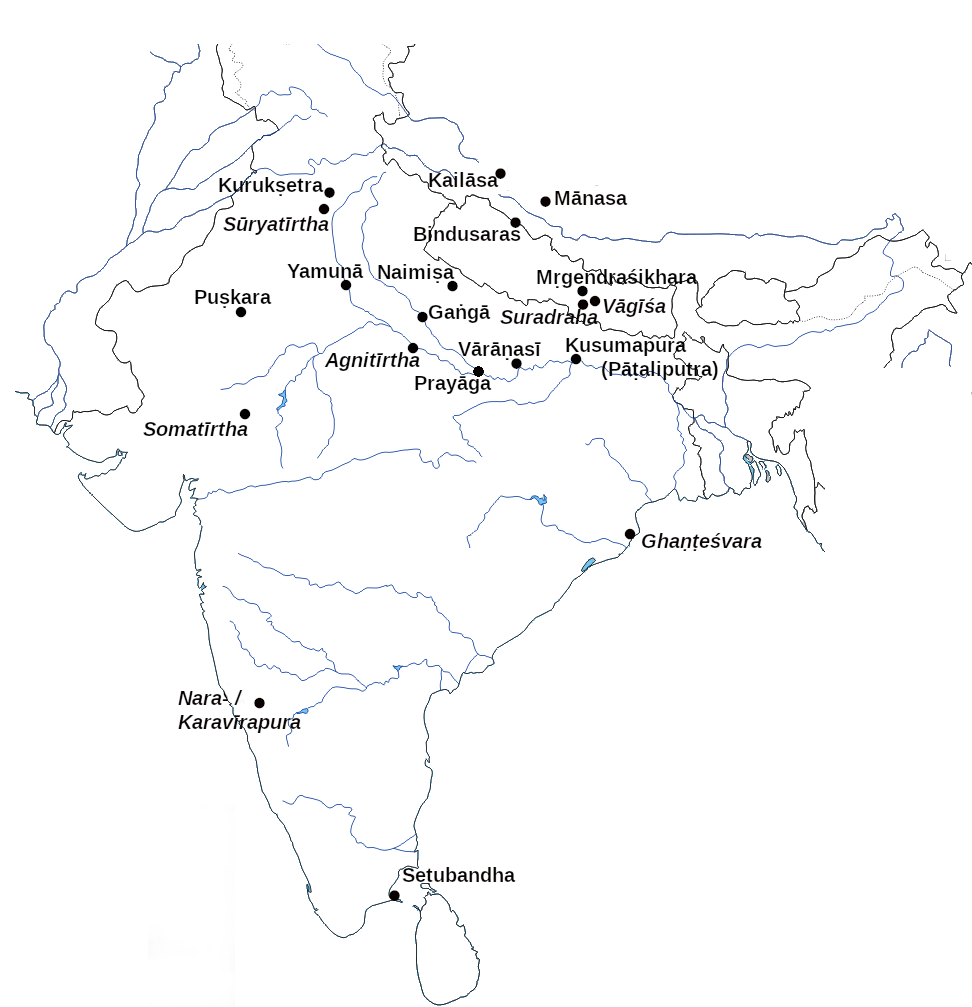
\includegraphics[scale=.5]{simplemap.png}

\caption{A possible reconstruction of the geography of the VSS. Toponyms in italics
are uncertain.
Map constructed using a simple hydrographic map made by Daniel Dalet (d-maps.com).}

\end{figure}

\leftskip0em\parindent2em


\vfill
\pagebreak




\subsection{Interpretation of chapters}

\begin{itemize}

\item
  Chapter 12

  \begin{itemize}
  
  \item
    everybody is donating to everybody,
  \item
    the final donor is Brahmā
  \item
    lot of testing going on in the frame story and also
  \item
    in chapter 12
  \item
    also the disguise thing is recurring: 12.37 and ch 1 and
  \item
    when Viṣṇu reveals his identity
  \end{itemize}
\end{itemize}









\subsection{The role of the VSS in the Śivadharma corpus}

\begin{itemize}
\item
  general ideas

  \begin{itemize}
  
  \item
    is this text really Śaiva? why in this collection?
  \item
    niśvāsa as sadāśiva in ch.~16; Niśvāsa uttarasūtra 5.50-51; see also
    Kafle Niśvāsamukha p.11ff; ibid. p.12: ``The term niśvāsa means
    sighing. Thus, an alternative meaning of the Niśvāsatattvasaṃhitā
    could also be a ``sighing tantra.'' To be more precise, a tantra
    that originated from the sighing of Śiva. This is to say, the speech
    of Śiva.''
  \item
    tattva-system: mati and suśira (ch.~20)
  \item
    parallels: MBh, Bṛhatkālottara,
  \item
    ch.~21: Viṣṇu; is this a Śaiva text?
  \item
    āśramas are in an order different from usual; compare this to NĀT;
    ``Variations on the āśrama-system''
  \end{itemize}
\item
  History of Dharmasastra 2.1 pp.~416ff on āśramas
\item
  \begin{enumerate}
  \def\labelenumi{\alph{enumi}.}
  \setcounter{enumi}{13}
  
  \item
    988! see Āpastamba-dharma-sūtra ii.9.21.1: catvāra āśramā
    gārhasthyam ācāryakulaṃ maunaṃ vānaprasthyam iti\textbar{} Quoted by
    Śankara But the chapters in Āpastamba follow the traditional order.
    ``Āp. places the householder first among the āśramas, probably on
    account of the importance of that stage to all other āśramas.'' Kane
    ibid.
  \end{enumerate}
\item
  ibid p.~417: person in last āśrama is called: parivrāṭ,
  parivrājaka(!), bhikṣu, muni, yati. See Olivelle, Patrick. The Āśrama
  System. The History and Hermeneutics of a Religious Institution. New
  York, Oxford: Oxford University Press, 1993. {[}megvan{]} p.82ff: The
  Order of Āśramas; ibid: ``In later texts the usual order is student,
  householder, hermit, and renouncer, reflecting the sequence of the
  passage from one \emph{āśrama} to another\ldots{} In the Dharmasūtras,
  however, only Baudhāyana and Vasiṣṭha follow that order\ldots{} A
  specific order becomes insignificant when the \emph{āśramas} are taken
  as four alternative adult vocations.'' Are they alternative adult
  vocations here in the Vṛṣasārasaṃgraha? They are numbered.
\item
  \textit{Gṛhastha. The Householder in Ancient Indian 
      Religious Culture.} Edited by Patrick Olivelle. OUP, 2019.
  Especially Csaba Dezső's article in it.
\item
  \%dscn 8034.jpg ff in folder
  /home/csaba/mmedia/images/scan/saiva/sivadharmacorpus/pasupatimatam4/
  \% in Naraharinātha's Paśupatimatam pp.~580ff \% CHECK if Naraharinath
  seems to be better at Sanskrit in other texts \% the edition seems
  problematic at many places \% a dialogue between Janamejaya and
  Vaiśampāyana, the latter of whom relates dialogues between Vigatarāga
  and Anarthayajña \% revise ¤s and lost/ill Bisschop in ``Universal
  Śaivism'': " -- En-dashes indicate a lost or illegible syllable in the
  manuscript."
\item
  \%N. of a celebrated king to whom Vaiśampāyana recited the {[}MBh.{]}
  (greatgrandson to Arjuna, as being son and, successor to Parikshit who
  was the son of Arjuna's son Abhimanyu) {[}"SBr.{]} xi, xīi AitBr.
  "Sāṅkhir. xvi {[}MBh.{]} \&c.;
\item
  \mycitep{BisschopUniversal2018}{2}: ``The full text of the corpus was first published by
  Naraharinātha in 1998, while over the past few years several scholars
  have started to work on individual parts of the corpus or referred to
  them in their studies. See, in particular, Acharya 2009; Bisschop
  2010, 2014; De Simini 2013, 2016a, 2016b, 2017; De Simini \& Mirnig
  2017; Goodall 2011; Kafle 2013, 2015; Magnone 2005; Sanderson 2003/04,
  2012/13; Schwartz 2012. An edition of the Śivadharmaśāstra alone,
  based on a single manuscript in the Adyar Library, has been published
  more recently as well (Jugnu \& Sharma 2014). The Śivopaniṣad, which
  also forms part of the Śivadharma corpus, was already published much
  earlier but was not recognised as such, being included in a collection
  of Upaniṣads (Kunhan Raja 1933).''
\item
  What MS did Naraharinātha used? See Biscchop 2018:58--59.
\item
  Palm leaf:
  /home/csaba/mmedia/images/scan/saiva/sivadharmacorpus/mss\_florinda/newari/ngmpp/palm\_leaf\_mtm/A
  3:3/fr.8493.0.A 0003-03\_3/A3-03+65851+177\_vss\_start.jpg Paper MS
  /home/csaba/mmedia/images/scan/saiva/sivadharmacorpus/mss\_florinda/newari/ngmpp/paper\_mtm/A
  1341-06/DSCN0331 fol.~204\_vss.JPG
\item
  Vipula

  Vipula in the MBh:

  MBh 13040016aff

  Devaśarman and his wife Ruci 13040017a tasya rūpeṇa --\textgreater{}
  13040017a tasyā rūpeṇa

\begin{quote}
  all gods, esp. Indra, are in love with her but Devaśarman guards her
  wants to perform yajña: how to guard her during the ritual?  calls his
  pupil, Vipula tells him that Indra can assume various forms Vipula
  decides that the only way to protect her from Indra is to magically
  'enter' her (with yoga) he tells her stories and enters her 

  MBh 13041001ff Indra sees the opportunity and enters the āśrama as a
  beautiful man he sees Vipula's lifeless body Ruci fancies Indra, but
  Vipula in his body stops her from standing up Indra sings to her
  beautiful songs he says "I have come for you, I am Devendra, I am in
  love" Vipula stops her from doing anything Indra is a bit shocked by
  her not being moved, gets angry and can see now that Vipula is in her
  Vipula leaves her, enters his own body, and abuses Indra and tells
  Indra how wicked he is Indra is ashamed and disappears Devaśarman
  returns to the āśrama, Vipula tells him what happened and Devaśarman
  praises him
\end{quote}
\item
  ETC., see translation here:
  https://www.sacred-texts.com/hin/m13/m13b005.htm
\item
\begin{quote}
  See summary also here:
 V. S. Sukthankar. Critical Studies in the Mahābhārata.  Poona, V. S.
 Sukthankar Memorial Edition Committee, 1944. 317--318
 https://archive.org/details/in.ernet.dli.2015.281344/page/n333
\end{quote}
\end{itemize}

\subsection{Dhyāna in the \VSS\ and the \DHARMP}

Compare, borrowings

\subsection{Misc}

\begin{itemize}
\item
  susūkṣma: Śivadharmottara 10.45cd--46: rudraḥ ṣaḍviṃśakaḥ proktaḥ
  śivaś ca paratas tataḥ \textbar{}\textbar{} 45 \textbar{}\textbar{}
  saptaviṃśatimaḥ śāntaḥ susūkṣmaḥ parameśvaraḥ \textbar{}
  svargāpavargayor dātā taṃ vijñāya vimucyate \textbar{}\textbar{} 46
  \textbar{}\textbar{}. yamas-niyamas: see table in 
  \mycitep{SaivaUtopia2021}{17}
\item
  other Why is this mentioned at
  http://cudlḷib.cam.ac.uk/view/MS-ADD-01694-00001/403 : C., Kunhan
  Raja, Un-published Upanishads (Adyar: The Adyar Library, 1933). Ahhh,
  Śivopaniṣat is in there! cf.~śivasaṃkalpa in pp 319 ff.
  (Śivasaṃkalpopaniṣat) Bonazzoli, Giorgio, ``Introducing Śivadharma and
  Śivadharmottara'', Altorientalische Forschungen vol.~20 issue. 2
  pp.~342-349 (1993). ``There is no raw data.'' EdX Harvard Digital
  Humanities
\item
  CHECK out Kenji on the Umāmaheśvarasaṃvāda in the MBh, his summary
  looks similar to the VSS
\item
  Kenji: `'BDhS 2: Discussion of gṛhastha. but BDh 2.11.9--34 is a
  digression on the topic of caturāśrama (vikalpa type, not krama type),
  and the author denies caturāśrama idea.''
\item
  MSS: see \mycitep{BisschopUniversal2018}{52--53}; 
  De Simini \& Mirnig
  pp.~587, 591 \% ``a stable element of the corpus''
\item
  Vindicate your edition: look at the apparatus, all the Ed entries
\end{itemize}




\subsection{Texts related to the \VSS}

MBh
Manu
Niśvāsakārikā

\vfill
\pagebreak


\subsection{Pāśupatas in the \VSS}

\subsection{Buddhism in the \VSS}

\vfill
\pagebreak

\subsection{Notes on the language}

\noindent
The language of the VSS goes beyond the idiosyncrasies of epic Sanskrit.
It exhibits strong similarities to Śaiva Aiśa Sanskrit,% 
		\footnote{See Goodall, Törzsök, Hatley, Kiss, Meyr?} 
and it applies particular metrical licences and 
uses a special vocabulary, morphology and syntax.
The analysis of this language, ideally, could lead us to the 
author(s) or redactors of the text and to its
place of composition. Here I only give a brief overview of the most
important phenomena. For details see the observatoins 
on the constitution of the Sanskrit text in the footnotes 
to the translation (pp. ??), as well as the Index.

\subsubsection{Newari?}

- \VSS\ too old for this comparison?

- metre?

- 

\subsubsection{Metre}
As regards metrical licences, the first striking feature is the generous
use of the poetic licence sometimes labelled `muta cum
liquida,'\footnote{For recent contributions on this phenomenon, see
  e.g.~Ranjan Sen 2006 (discussing it as appearing in Latin) and Balogh
  2018, note 6 (discussing Sanskrit metre).} namely that some consonant
clusters that would normally turn the previous short (laghu) syllable
long (guru) may in some cases do not do so. The syllables pra, bra, hra,
kra, especially at the beginning of words CHECK, are well-known
candidates for this licence.\footnote{See e.g.~Apte' XXX Dictionary
  Appendix A p.~1. ADD real life examples.} In the VSS, tra, vra, śra,
pra, and also śya, śva, sva, dva, all involving conjunct consonants with
a liquid sounds or semi-vowels in second position, and possibly also
rpa,CHECK! seem additional ones.

Parākhya 5:4c, 5:44a, 5:76c, 5:124a. (see p. lxxxi)

SYM: pūjayet ... mantriṇā 18.23 b-d;
yajec cakre ca vidhivad yoginīsiddhim icchatā 21.12cd


The well-known author on prosody, Kedārabhaṭṭa (11-12th centuries),%
		\footnote{SOURCE}	 
frequently quoted by Mallinātha, gives the following definition in his
\skttitle{Vṛttaratnākara}{Vrttaratnakara} (here given together with Sulhaṇa's \skttitle{Sukavihṛdayanandinī}{Sukavihrdayanandini} commentary):

\begin{quote}
\emph{padādāv iha varṇasya saṃyogaḥ kramasaṃjñikaḥ} \textbar{}\\
\emph{puraḥsthitena tena syāl laghutā 'pi kvacid guroḥ}
\textbar{}\textbar{} 1.10 \textbar{}\textbar{}
\end{quote}

\begin{quote}
\begin{quote}
\emph{vibhaktyantaṃ padaṃ tasya padasyādau vartamāno yo varṇas tasya
saṃyogaḥ} \textbar{} \emph{sa iha śāstre kramasaṃjño jñeyaḥ} \textbar{}
\emph{tena krameṇa purovartinā prākpadānte vartamānasya
prāptagurubhāvasyāpi laghutā syāt} \textbar{} \emph{kvacil
lakṣānurodhena} \textbar{} \emph{nanu ka eṣaḥ kramo nāma saṃyoga ucyate}
\textbar{} \emph{pūrvācāryāṇāṃ piṅgalanāgaprabhṛtīnāṃ kālidāsādīnāṃ ca
kavīnāṃ samayaḥ parigṛhītaḥ} \textbar{} \emph{saṃyogaḥ kramasaṃyogaḥ}
\textbar{}\textbar{} 10 \textbar{}\textbar{} \emph{tatra gra-saṃyogena
yathā} \textbar{} \emph{idam asyodāharaṇam} \textbar{}
\end{quote}
\end{quote}

\begin{quote}
\emph{taruṇaṃ sarṣapaśākaṃ navaudanaṃ picchalāni ca dadhīni}
\textbar{}\\
\emph{alpavyayena sundari grāmyajano miṣṭam aśnāti} \textbar{}\textbar{}
1.11 \textbar{}\textbar{}
\end{quote}

TRANSLATE the whole passage!

\begin{quote}
In this {[}work{]}, a consonant cluster at the beginning of a word is
called krama. A {[}preceding{]} long syllable can sometimes be turned
short by that initial {[}syllable{]}.
\end{quote}

\begin{quote}
\begin{quote}
\begin{quote}
   ... TRANSLATE 
\end{quote}
\end{quote}
\end{quote}

\begin{quote}
Tender mustard seed, fresh porridge, and slimy curds: village people eat
this kind of dishes, O beautiful goddess, due to lack of money.
\end{quote}

To sum this example up: the verse given above (1.11) is in āryā, and the
metric pattern of the second half-verse is the following: - - . - . - .
- - . . - - . - - - This yields 28 morae, instead of the expected 27. By
treating the final syllable of sundari short, in spite of the following
grā, the pattern conforms to the expected pattern: - - . - . - . . - . .
- - . - - -

The commentator gives several more examples (involving the syllables
gra, hra, bhra), including this Śārdūla line:

\begin{quote}
nidravyo hriyam eti hrīparigataḥ prabhraśyate tejasaḥ
\end{quote}

In this line, the last syllable of eti should count as short, in spite
of the fact that the beginning of the next word (hrī°) would normally
turn it long.

The VSS abounds in this phenomenon of `muta cum liquida'. EXAMPLES from
the VSS and from my emendations. CHECK

\begin{itemize}
\item
  only beginning of words in the VSS?
\item
  final -am etc. counts as long (reverse of muta cum liquida)
\item
  In Kannada and Telugu prosody, under the name of śithila-dvitva, the
  exception is that sometimes in a consonant cluster of the form
  {[}consonant + ``r''{]}, the ``r'' (repha) can be ignored, so that it
  is not a conjunct consonant anymore.
\item
  The exception is not accepted by purists: Shatavadhani Ganesh says
  that the Sanskrit masters like Kālidāsa, Bhāravi, Māgha, Śrīharṣa, and
  Viśākhadatta have not freely used this exception (though the masters
  in Kannada and other languages have). Being more of a ``poetic
  licence'' and a violation of the standard rule (only found in later
  poetry), it is extremely unlikely that any sane poet would have
  indulged in that exception in all four pāda-s of a verse. Thus it is
  very unlikely that the program will miss identifying a verse that
  indulges in this
\item
  Reference: see comments by Dr.~Ganesh and Nityananda Misra in this
  thread started by Vishvas Vasuki:
  \%https://groups.google.com/forum/\#!topic/bvparishat/ya1cGLuhc14/discussion
  
  poetic licences
\end{itemize}


\subsubsection{Vocabulary}

\begin{itemize}

\item
  Special vocabulary/language: karhacit, hṛdi as nominative 10.27cd,
  tirya, me as mayā, āhūtaplavana
\item
  generate list from index
\end{itemize}


\subsubsection{Number and gender}

\begin{itemize}

\item
  Number: singular next to numerals, and general confusion (CHECK)

\item the more original a section the more extreme language? see ch11
\end{itemize}


\subsubsection{Syntax}

\begin{itemize}

\item
  Special structures: caturmaunasya vakṣyāmi indreṇāsmi phalaṃ dattaṃ
\end{itemize}

kathito 'smi

as if not proofread

\subsubsection{Stem form nouns}

\begin{itemize}
\item
  stem form nouns (prātipadika); 
  \mycitep{NewariGrammar}{\S 18.1}: `Nominative. This case has no ending but represents the pure stem.'
\item
  a more or less full collation is important: we cannot automatically
  reject `ungrammatical' or unmetrical forms because they may well be
  the `original' one
\end{itemize}




\vfill
\pagebreak

